\chapter{Webauftritt}
\renewcommand{\kapitelautor}{Autor: Hatice Akyokus}
In diesem Kapitel wird der Webauftritt erläutert. Der Webauftritt ist der wichtigste Bestandteil der Diplomarbeit, da sich alle Elemente auf dieser befinden.
 
\section{Nutzen und Inhalt}
Um die Zielgruppe am Besten zu erreichen, wurde eine Webseite erstellt. Diese soll zeigen, was in den fünf Jahren Medientechnik beigebracht wird. Weiters soll sie Missverständnisse beseitigen und dafür sorgen, dass Interessenten so gut wie möglich informiert sind. Dafür beinhaltet die Webseite eine Startseite, welche kurz und knapp den Inhalt der Webseite erklärt, interaktive Elemente und Videos, die einerseits informieren und andererseits den Spaßfaktor der Webseite erhöhen sollen. 

\section{Bildquellen}
Alle verwendeten Bilder, wurden von der Webseite unsplash.com heruntergeladen. Unsplash.com ist eine Webseite, auf der User ihre eigenen Bilder hochladen können. Diese können von anderen Usern kostenlos heruntergeladen werden. Weiters wurden kostenlose Vektorgrafiken von der Webseite flaticon.com verwendet. Dies ist eine Webseite, welches Vektorgrafiken in verschiedenen Formaten anbietet. Es gibt kostenpflichtige und kostenfreie Grafiken, die frei anpassbar sind. Im Rahmen der Diplomarbeit wurden Bilder verwendet, die dem Corporate Design entsprechen und zu dem Thema der Diplomarbeit passen. Das Team entschied sich für ein „Space-Theme“, welches die Größe der Medientechnik grafisch darstellen sollte. 

\section[Frameworks und Libraries]{Frameworks und Libraries\protect\footnote{\label{foot:2}vgl.https://www.eins2design.de/blog/168-was-bedeutet-framework-und-wozu-wird-es-verwendet [Zugriff: 18.03.2018]}} 
Framework heißt übersetzt Rahmenkonstruktion und wird häufig bei Webseiten verwendet. Sie dienen als Gerüst zum Programmieren und erleichtern die Arbeit, die damit verbunden ist. Dabei ist das Framework selbst kein Programm, sondern ein Rahmen, welcher den Inhalt ansprechend präsentiert. Bei den CSS-Frameworks standen dem Team Foundation und Bootstrap zur Auswahl. Es wurde im Internet nach einer Pro und Contra Liste gesucht und beide Frameworks wurden verglichen. Obwohl Bootstrap bekannter ist, hat sich das Team dennoch für Foundation entschieden, da mit Foundation entwickelte Webseiten ansprechender wirken und jene mit Bootstrap gleich aussehen. Außerdem bietet Foundation einen fluiden Ansatz, wenn es um Responsiveness geht. Bei Bootstrap müssten noch weitere Zeilen an Code geschrieben werden, um einen fluiden Ansatz anzustreben.   Weiters kann Foundation nach Belieben angepasst werden, ohne, dass sie anderen Webseiten ähnelt. Allerdings ist ein Nachteil, dass die Community ziemlich klein ist. Somit kann nicht schnell nach einer Lösung im Internet gesucht werden, man muss sich selbst etwas überlegen. Im Rahmen der Diplomarbeit wurden mehrere Frameworks für die Webseite verwendet. Es wurde ein CSS-Framework verwendet, welches dafür sorgt, dass die Webseite responsiv ist. Weiters wurden mehrere Javascript und jQuery-Frameworks verwendet, welche für die interaktiven Elemente verwendet wurden, da sie erweiterte Funktionen bieten. 

\subsection[Foundation]{Foundation\protect\footnote{\label{foot:2}vgl.https://foundation.zurb.com [Zugriff: 27.03.2018]}}
Foundation ist ein CSS-Framework, welches entwickelt wurde, um die Webseite responsiv und modern zu gestalten. Das Prinzip von Foundation liegt darin, die programmierte Webseite auf allen Endgeräten identisch aussehen zu lassen. Dieses Prinzip nennt sich mobile-first. Foundation kann entweder heruntergeladen oder per CDN eingebunden werden. Das Team entschied sich dazu, das Framework herunterzuladen. Während eine CDN eine verringerte Reaktionszeit hat, kann sie nicht optimiert werden. Lokal gespeicherte Daten hingegen können jederzeit bearbeitet und den Wünschen des Teams angepasst werden. Somit wurde Foundation von der Webseite foundation.zurb.com heruntergeladen und lokal eingebunden. Dadurch konnte das Team Änderungen in der CSS-Datei vornehmen. 
\subsection{Slick Slider}
Slick slider ist ein Framework, welche hauptsächlich für Slider gedacht ist. Da die Webseite dieser Diplomarbeit auf diesem Prinzip beruht, entschied sich das Team dazu, slick slider zu verwenden. Der Entwickler dieses Frameworks wirbt für slick mit folgendem Slogan: „slick – the last carousel you’ll ever need“ . Slick ist sehr einfach zu bedienen, da die Programmierarbeit sehr minimal ist. Die nötigen Methoden werden bereits vom Framework angeboten, wobei man sehr viel anpassen kann. Somit muss man die vordefinierten Klassen nicht verwenden und kann es vom Aufbau her, so gestalten wie man möchte. Dies wurde in der Diplomarbeit natürlich ausgenutzt um die Webseite einzigartig erscheinen zu lassen. Slick bietet dem Nutzer sehr viele Möglichkeiten an, die Slider zu steuern oder zu gestalten und ist responsive und basiert ebenfalls auf dem mobile-first Prinzip. Außerdem bietet slick den Nutzern die Möglichkeit, Breakpoints zu setzen.
\begin{figure}[H] 
  \centering
     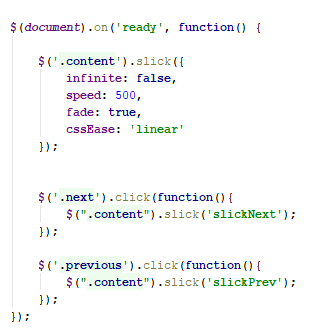
\includegraphics[width=0.7\textwidth]{webseite_abb1.png}
  \caption{Aufruf von Slick Slider}

\end{figure}

Wie man in der Abbildung sehen kann, wird slick aufgerufen. Es können vordefinierte Parameter übergeben werden, welche man nach Belieben einstellen kann. Das Team hat außerdem eigene Weiterschalt-Buttons definiert, welche sich nicht, traditionell wie bei anderen Slidern, links und rechts befinden, sondern unterhalb. Slick wurde ebenfalls heruntergeladen und lokal hinzugefügt. 

\section{Responsiveness}
Um zu gewährleisten, dass die Webseite auf allen Endgeräten einwandfrei funktioniert, wurde auf die Responsiveness einen sehr großen Wert gelegt. Vor allem, da die Webseite sehr viele Bilder enthält.

\begin{quote}
Responsive Webdesign ist kein Trend! Studien zum Absatz mobiler Endgeräte belegen eine stetige Zunahme der Verkäufe von Tablets und Smartphones. Diese Entwicklung wird nicht nur von der Fachszene mit Euphorie verfolgt, es gibt auch fast täglich neue Entwicklungen zum Thema der technischen und grafischen Umsetzung von Webseiten für mobile Endgeräte. Responsive Webdesign spielt mit der geräteübergreifenden Flexibilität eine tragende Rolle in dieser Bewegung die sich zunehmend zu einem Standard entwickelt. 
\end{quote}

Durch Responsive Design wird eine bessere Bedienbarkeit gewährleistet und somit die Bounce-Rate deutlich reduziert. Außerdem ergibt sich weniger Wartungsaufwand bei Updates.  Das CSS-Framework hilft dabei als Gerüst, die Webseite responsiv zu machen. Allerdings muss auch nachgeholfen werden und dies erfolgte hauptsächlich mit Flexbox. Dies ist eine sehr einfache Möglichkeit, flexible Layouts zu erstellen, ohne CSS-Einstellungen wie position zu verwenden. In der Diplomarbeit wurde sie hauptsächlich dafür verwendet, Elemente zu zentrieren, denn dies erweist sich, vor allem für das vertikale Zentrieren von Elementen, als kompliziert. 

\begin{figure}[H] 
  \centering
     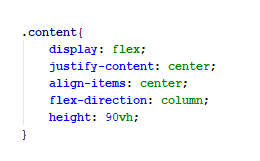
\includegraphics[width=0.7\textwidth]{webseite_abb2.png}
  \caption{Anwendung von Flexbox}

\end{figure}

Wie in der Abbildung zu erkennen ist, wird auf das Element mit der Klasse content, eine Flexbox angewendet. Alle Kindelemente von content werden, sowohl horizontal als auch vertikal zentriert angezeigt. Außerdem wurden bei den Größenangaben keine Werte in Pixel angegeben. Das Pixel ist eine absolute CSS Einheit und darin liegt auch das Problem, denn sobald die Webseite verkleinert wird, bewegt sich der Inhalt nicht mit und ist somit nicht responsiv. Deswegen wurden relative CSS Einheiten, wie vw, vh und rem verwendet. Die Einheiten vw und vh stehen für viewport width und viewport height und entsprechen dem 100. Teil der Breite des Anzeigebereiches. Allerdings werden sie vom Internet Explorer erst ab Version 9 unterstützt. Die Einheiten viewport width und viewport height wurden für Div-Boxen verwendet, da es wichtig ist, dass sie responsiv sind.  Für Schriftarten wurde rem, root em, verwendet. 

\begin{quote}
„rem verhält sich genauso wie em mit dem einzigen Unterschied, dass das sich der rem-Wert am Root-Element orientiert (also an der Schriftgröße, für body bzw. html), statt sich wie em an der Schriftgröße des jeweiligen Eltern-Elements zu orientieren.“
\end{quote}

Da rem nicht von älteren Browsern unterstützt wird, musste eine Fallback-Lösung in px im Stylesheet definiert werden.   Außerdem wurden Breakpoints eingearbeitet, um eine Responsiveness, vor allem für mobile Geräte, zu gewährleisten. 

\subsection{Startseite}
Die Startseite ist eine entscheidende Seite, welche das Interesse anregen soll. Es war dem Team sehr wichtig, die Startseite so modern wie möglich zu gestalten, um den User dazu zu bringen die Webseite zu erkunden. Auf der Navigationsleiste befindet sich das Logo und weitere Links, Über Uns, Download, Kontakt und ein FAQ. Diese sind sehr simpel gehalten. Die Navigationsleiste ist schlicht gehalten und weiß. Die Schrift ist in dem orange des Corporate Designs und wenn man mit der Maus über die Links fährt, werden sie grün. 

\begin{figure}[H] 
  \centering
     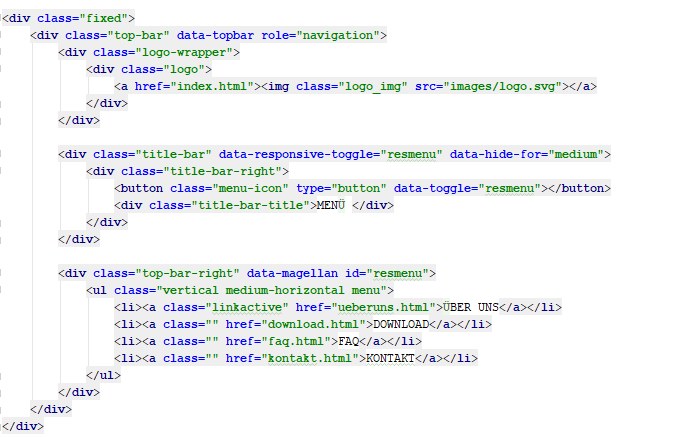
\includegraphics[width=0.7\textwidth]{webseite_abb3.png}
  \caption{Aufbau der Navigationsleiste}

\end{figure}

Die Navigation besteht aus drei Containern, wobei eines das Logo enthält, eines welches bei Verkleinern des Bildschirms einen Menü-Burger erscheinen lässt und eines, welche die Links zu den erwähnten Links enthält. Die Klasse „linkactive“, hebt die Seite, auf der man sich gerade befindet, hervor. 
\\
Die Seite Über Uns, gibt dem User Informationen über die Entwickler der Webseite und den Nutzen den diese hat. Sie ist, wie alle anderen Links, im Space-Theme gehalten. \\
Weiters kann man ein Dokument, welches zusätzliche Informationen über die Medientechnik enthält und zur Webseite ergänzend wirken soll, herunterladen. Dieses ist sehr detailliert und ist auch für die Eltern der Schüler gedacht, um soviel Informationen, wie möglich über die Medientechnik zu bekommen.
\\
Bei Fragen, kann auf die Kontaktseite wechseln, welches ein Kontaktformular enthält, was das Kontaktieren der Schule vereinfachen soll. Außerdem befinden sich auf dieser Seite auch Kontaktinformationen der Schule, falls es User präferieren die HTL anzurufen. \\
Der User hat allerdings auch die Möglichkeit, in das FAQ (Frequently Asked Questions) einen Blick zu werfen, auf der sich häufig gestellte Fragen befinden. Somit entlastet man diejenige Person, die sich um die Fragen kümmert. Die Fragen wurden am Tag der offenen Tür gesammelt und auch selbst ausgedacht. 

\section[Storytelling]{Storytelling\protect\footnote{\label{foot:2}vgl. https://www.textbroker.de/storytelling [Zugriff: 18.03.2018]}}

\begin{quote}
Kinder verpacken Ihre Ideen und Gedanken oftmals in Geschichten, um uns Erwachsene damit ihre Welt zu erklären. Als Erwachsene wiederum müssen wir es wieder lernen, Geschichten zu erzählen.
\end{quote}
Storytelling vermittelt durch den Einsatz von Geschichten Information. Die Geschichten können real oder konstruiert sein, es muss lediglich gut ankommen und im Kopf der Nutzer bleiben. Weiters dient Storytelling dazu, die Aufmerksamkeit des Nutzers zu ergattern und das auf eine kreative Weise. Die Informationen werden dabei anschaulich gemacht, um die Botschaft ankommen zu lassen. Wichtig ist die Erstellung eines oder mehreren Protagonisten und einem Problem. Im Laufe der Geschichte, soll sich das Problem lösen oder auch nicht. Eine gute Geschichte führt dazu, dass sich die Nutzer mit der Thematik auseinandersetzen und emotional aufgeladen sind. Weiters sorgt eine gute Story für Begeisterung. Es gibt verschiedene Arten von Storytelling, vom Buch bis hin zu Werbevideos und Webseiten. Das Internet bietet hier eine große Möglichkeit für das Erzählen von Geschichten. Wichtig ist vor allem die Interaktivität, damit es nicht zu schnell langweilig wird.  Für das Team war es wichtig, die Zielgruppe durch die Geschichte zu erreichen. Dabei sollten Klischees vermieden werden und die Nutzer sollten sich mit dem Erzähler identifizieren können. 

\subsection{Story}
Project Insight benutzt klassische Storytelling-Methoden, um Nutzer über die Medientechnik zu informieren. Dabei dachte sich das Team, die Figur, Rene Weg, aus. Dieser ist ein Absolvent der HTL Rennweg und hat dem Nutzer gegenüber eine Mentor-Funktion. Rene Weg, ist eine sarkastische und humorvolle Figur, welcher dem Nutzer die Medientechnik, auf eine spielerische und lockere Art und Weise, präsentiert. Es war dem Team sehr wichtig, ein paar Witze in die Story einzubinden, um dem Nutzer das Gefühl zu geben, dass man an der HTL Rennweg auch Spaß haben kann. Durch verschiedenste Gestiken und Mimik, wird Leben in die Figur gehaucht. 

Abgesehen von der Rolle der Figur als Mentor, kommt sie auch noch in dem Animationsvideo (siehe Kapitel Animationsvideo) vor. 

\subsubsection{Aufbau}
Die Story ist in zehn Kapitel aufgeteilt. Dabei arbeitet sich der User stufenweise in die Medientechnik ein. Es beginnt mit einer Einführung und geht Schritt für Schritt die vorgegebenen Bereiche der Medientechnik durch und endet anschließend mit einem humorvollen Video. Bevor die Story beginnt, wird der User darauf hingewiesen, dass die Webseite Audio beinhaltet. Die Webseite wird vom Charakter, Rene Weg, vertont. 
Für das Grundgerüst wurde das Framework slick slider verwendet. Dabei wurde ein Grid erstellt, wo sich auf einer Seite der Text und auf der anderen Seite die Figur befindet. 

Zusätzlich befinden sich unter dem Text vier Buttons, welche für das Weiterschalten und für das Pausieren und Abspielen gedacht sind. 

\begin{figure}[H] 
  \centering
     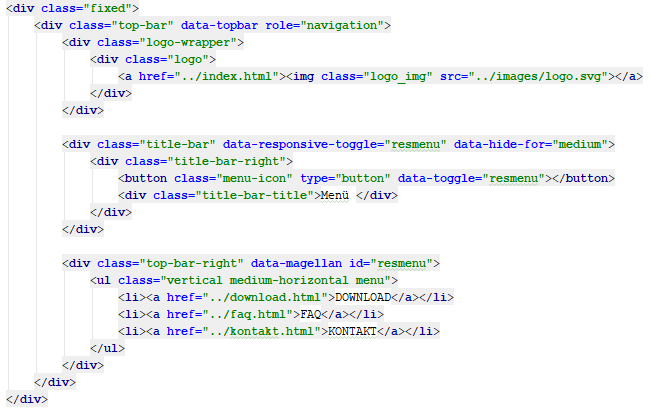
\includegraphics[width=0.7\textwidth]{webseite_abb4.png}
  \caption{Aufbau einer Slide}
  
  \centering
  	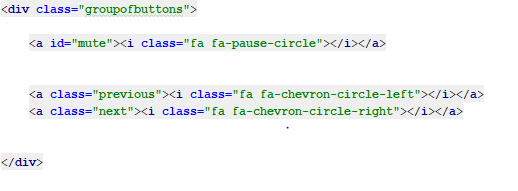
\includegraphics[width=0.7\textwidth]{webseite_abb5.png}
  \caption{Aufbau der Weiterschalt-Buttons}

\end{figure}

In den beiden Abbildungen ist die Struktur der Webseite zu sehen. Jedes Slide hat eine eigene ID und hat zwei Kindelemente, welche sich jeweils links und rechts befinden und den Text und die Figur beinhalten. Das Element mit der Klasse „groupofbuttons“ beinhaltet die Buttons mit denen man zum nächsten Slide gelangt. Klickt man auf die Weiterschalt-Buttons, kommt man zum nächsten Slide. Sobald man auf den Pause-Button klickt, wird das Audio pausiert und kann durch den Play-Button wieder abgespielt werden. Will man sich das Audio noch einmal anhören, so kann man ebenfalls auf den Play-Button klicken. Die große Problematik beim Aufbau war es, pro Slide ein einziges Audio-File abzuspielen. Öfters ist es vorgekommen, dass beim Weiterklicken, das vorherige Audio-File noch mitspielt. Um dies zu verhindern, wurden if-Statements eingebaut, welche überprüfen, ob sich der User in einem bestimmten Slide befinden. Befindet sich der User beispielsweise im zweiten Slide, wird das zugehörige Audio-File abgespielt. Sobald man das zweite Slide verlässt, pausiert sich das Audio-File, so dass sich keine Audio-Files überkreuzen. 

\begin{figure}[H] 
  \centering
     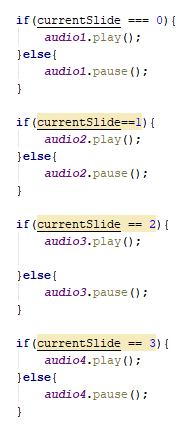
\includegraphics[width=0.7\textwidth]{webseite_abb6.png}
  \caption{Die if-Statements sorgen für ein reibungsloses Abspielen der Audio-Files}

\end{figure}

Nicht jedes Slide hat ein Audio-File, da es Slides gibt, welche dem Nutzer darüber informieren, welche Lektion gerade bearbeitet wird. Bei diesen Slides, ändert sich die Struktur, denn die Play und Pause-Buttons verschwinden und die Weiterschalt-Buttons rücken in die Mitte. Außerdem gibt es Slides, welche Videos beinhalten und nicht vertont wurden, welche ebenfalls keine Play und Pause-Buttons enthalten.

Am Ende der Lektion, wurde dem Weiterschalt-Button ein Link zur nächsten Lektion hinzugefügt. 

Hierbei wird der letzte Slide ermittelt und dem Weiterschaltbutton ein Link hinzugefügt. Dies könnte einfacher programmiert werden, in dem man, ein if-Statement schreibt, welches nach dem currentSlide fragt aber dadurch, dass es zehn Lektionen gibt und es zusätzliche Arbeit wäre, dass bei Änderungen andauernd zu ändern. Durch die im Bild abgebildete Methode, muss pro HTML-Dokument nur der Link zum nächsten HTML-Dokument angegeben werden. \\
In den folgenden Absätzen, werden alle Kapitel zusammengefasst.

\paragraph{Kapitel 1}
In dem ersten Kapitel werden Fragen rund um die HTL beantwortet. Am Anfang stellt sich die Figur vor und zeigt dem User anschließend ein Animationsvideo, welches erklärt, was eine HTL ist und was die HTL Rennweg bietet.
\paragraph{Kapitel 2}
Im zweiten Kapitel, stellt die Figur den Abteilungsvorstand der HTL Rennweg, Dr. Gerhard Hager, vor. Bevor das Interview gezeigt wird, erklärt der Charakter kurz und knapp, was ein Abteilungsvorstand ist.
\paragraph{Kapitel 3}
Im dritten Kapitel wird die Medientechnik erklärt. Der Charakter steht in diesem Kapitel im Vordergrund und interagiert mit dem Nutzer und plaudert über die Medientechnik. Dabei vergleicht er die Größe der Medientechnik mit dem Universum und bezieht sich somit auf das „Space-Theme“, welches konsistent auf alle Seiten der Webseite durchgezogen wurde. 
\paragraph{Kapitel 4}
Im vierten Kapitel geht es um die Mediengestaltung. Dabei erklärt Rene Weg dem User, wie wichtig es ist langweiligen Inhalt, spannend zu gestalten. Als Beispiel wird die Entstehungsgeschichte der HTL aufgelistet und danach wird eine spannendere Auflistung hergezeigt. Dieses Kapitel dient dazu, dem User zu zeigen, wie wichtig Kreativität in der Medientechnik ist und dass man mit seinem Inhalt hervorstechen muss, um erfolgreich zu sein.
\paragraph{Kapitel 5}
Im fünften Kapitel werden Spiele thematisiert. Viele Interessenten, interessieren sich für die Entwicklung von Spielen und sehen ein paar bei den Diplomarbeiten am Tag der offenen Tür. Das Team hat sich dabei dazu entschieden, den Code herzuzeigen. Damit der Code kurz und knapp ist und nicht zu kompliziert wirkt, da die User keine Erfahrung damit gemacht haben, hat sich das Team für das Spiel Memory entschieden. Nachdem der Code gezeigt wird, kann der User das Spiel auch spielen.
\paragraph{Kapitel 6}
Im sechsten Kapitel stehen Animationen im Vordergrund. Dabei kann der User, sein eigenes Universum kreieren. Dies erfolgt durch das Verschieben von Planeten und einer Rakete, welche in den Farben des Corporate Designs gehalten wurden. 
\paragraph{Kapitel 7}
Im siebten Kapitel geht es um Schrödingers Katze. Die Idee dahinter war, eine beliebte Referenz einer Fernsehserie, in ein interaktives Element umzuwandeln. In der Fernsehserie, The Big Bang Theory, gibt es eine Folge, in der Schrödingers Katze erwähnt wird und diese Folge ist sehr populär. Dies nahm das Team als Inspiration und programmierte eine Kiste, die geschlossen zu sein scheint. Fährt man mit der Maus über die Kiste, so sieht man eine weiße Katze. Dieses Kapitel unterstreicht, dass Kreativität sehr wichtig in der Medientechnik ist.
\paragraph{Kapitel 8}
Im achten Kapitel geht es wieder um die Medientechnik im Allgemeinen. Dabei hat das Diplomarbeitsteam den Medientechniklehrer und Medientechnikfachmann, Mag. Roman Jerabek, interviewt. In dem Interview wird die Medientechnik besprochen und ihre Wichtigkeit hinterfragt.
\paragraph{Kapitel 9}
Im neunten Kapitel können User sehen, was andere Interessenten über die Schule denken. Dies soll dazu dienen, die Entscheidung der User zu erleichtern, da sie die Meinung von anderen Interessenten hören.
\paragraph{Kapitel 10}
Im letzten Kapitel verabschiedet sich Rene Weg vom User. Doch bevor die Reise zu Ende ist, gibt es noch ein Bonus-Video. Die Intention dieses Videos ist zu zeigen, was ein Absolvent der HTL Rennweg beherrscht und was ein Schüler der zweiten Klasse, alles in so kurzer Zeit gelernt hat. Durch den Kontrast zwischen dem Absolventen und dem Schüler, soll klargemacht werden, dass wenn man in die Medientechnik geht andere Interessen hat und das nicht jeder Schüler gleich ist.\\
In dem folgenden Absatz werden die technischen Aspekte der interaktiven Elemente erläutert.

\subsection{Interaktive Elemente}
Storytelling funktioniert nicht ohne Interaktivität.  Dafür entwickelte das Team vier interaktive Elemente, welche einen Einblick in die Medientechnik geben. 
\subsubsection{Timeline}

\subsubsection{Memory}
Das Memory-Spiel kommt 

\subsubsection{Animationen}

\subsubsection{Schrödingers Katze}


